\documentclass[12pt]{beamer}
\usepackage{../Estilos/BeamerMAF}
\usetheme{Warsaw}
\usecolortheme{seahorse}
%\useoutertheme{default}
\setbeamercovered{invisible}
% or whatever (possibly just delete it)
\setbeamertemplate{section in toc}[sections numbered]
\setbeamertemplate{subsection in toc}[subsections numbered]
\setbeamertemplate{subsection in toc}{\leavevmode\leftskip=3.2em\rlap{\hskip-2em\inserttocsectionnumber.\inserttocsubsectionnumber}\inserttocsubsection\par}
\setbeamercolor{section in toc}{fg=blue}
\setbeamercolor{subsection in toc}{fg=blue}
\setbeamercolor{frametitle}{fg=blue}
\setbeamertemplate{caption}[numbered]

\setbeamertemplate{footline}
\beamertemplatenavigationsymbolsempty
\setbeamertemplate{headline}{}


\makeatletter
\setbeamercolor{section in foot}{bg=gray!30, fg=black!90!orange}
\setbeamercolor{subsection in foot}{bg=blue!30}
\setbeamercolor{date in foot}{bg=black}
\setbeamertemplate{footline}
{
  \leavevmode%
  \hbox{%
  \begin{beamercolorbox}[wd=.333333\paperwidth,ht=2.25ex,dp=1ex,center]{section in foot}%
    \usebeamerfont{section in foot} \insertsection
  \end{beamercolorbox}%
  \begin{beamercolorbox}[wd=.333333\paperwidth,ht=2.25ex,dp=1ex,center]{subsection in foot}%
    \usebeamerfont{subsection in foot}  \insertsubsection
  \end{beamercolorbox}%
  \begin{beamercolorbox}[wd=.333333\paperwidth,ht=2.25ex,dp=1ex,right]{date in head/foot}%
    \usebeamerfont{date in head/foot} \insertshortdate{} \hspace*{2em}
    \insertframenumber{} / \inserttotalframenumber \hspace*{2ex} 
  \end{beamercolorbox}}%
  \vskip0pt%
}
\makeatother

\makeatletter
\patchcmd{\beamer@sectionintoc}{\vskip1.5em}{\vskip0.8em}{}{}
\makeatother

\newlength{\depthofsumsign}
\setlength{\depthofsumsign}{\depthof{$\sum$}}
\newcommand{\nsum}[1][1.4]{% only for \displaystyle
    \mathop{%
        \raisebox
            {-#1\depthofsumsign+1\depthofsumsign}
            {\scalebox
                {#1}
                {$\displaystyle\sum$}%
            }
    }
}
\def\scaleint#1{\vcenter{\hbox{\scaleto[3ex]{\displaystyle\int}{#1}}}}
\def\scaleoint#1{\vcenter{\hbox{\scaleto[3ex]{\displaystyle\oint}{#1}}}}
\def\bs{\mkern-12mu}

\usepackage{courier}
%\usepackage{listingsutf8}
\usepackage{listings}
\usepackage{xcolor}
\usepackage{textcomp}
\usepackage{color}
\definecolor{deepblue}{rgb}{0,0,0.5}
\definecolor{brown}{rgb}{0.59, 0.29, 0.0}
\definecolor{OliveGreen}{rgb}{0,0.25,0}
% \usepackage{minted}

\DeclareCaptionFont{white}{\color{white}}
\DeclareCaptionFormat{listing}{\colorbox{gray}{\parbox{0.98\textwidth}{#1#2#3}}}
\captionsetup[lstlisting]{format=listing,labelfont=white,textfont=white}
\renewcommand{\lstlistingname}{Código}


\definecolor{Code}{rgb}{0,0,0}
\definecolor{Keywords}{rgb}{255,0,0}
\definecolor{Strings}{rgb}{255,0,255}
\definecolor{Comments}{rgb}{0,0,255}
\definecolor{Numbers}{rgb}{255,128,0}

\makeatletter

\newif\iffirstchar\firstchartrue
\newif\ifstartedbyadigit
\newif\ifprecededbyequalsign

\newcommand\processletter
{%
  \ifnum\lst@mode=\lst@Pmode%
    \iffirstchar%
        \global\startedbyadigitfalse%
      \fi
      \global\firstcharfalse%
    \fi
}

\newcommand\processdigit
{%
  \ifnum\lst@mode=\lst@Pmode%
      \iffirstchar%
        \global\startedbyadigittrue%
      \fi
      \global\firstcharfalse%
  \fi
}

\lst@AddToHook{OutputOther}%
{%
  \lst@IfLastOtherOneOf{=}
    {\global\precededbyequalsigntrue}
    {}%
}

\lst@AddToHook{Output}%
{%
  \ifprecededbyequalsign%
      \ifstartedbyadigit%
        \def\lst@thestyle{\color{orange}}%
      \fi
    \fi
  \global\firstchartrue%
  \global\startedbyadigitfalse%
  \global\precededbyequalsignfalse%
}

\lstset{ 
language=Python,                % choose the language of the code
basicstyle=\footnotesize\ttfamily,       % the size of the fonts that are used for the code
numbers=left,                   % where to put the line-numbers
numberstyle=\scriptsize,      % the size of the fonts that are used for the line-numbers
stepnumber=1,                   % the step between two line-numbers. If it is 1 each line will be numbered
numbersep=5pt,                  % how far the line-numbers are from the code
backgroundcolor=\color{white},  % choose the background color. You must add \usepackage{color}
showspaces=false,               % show spaces adding particular underscores
showstringspaces=false,         % underline spaces within strings
showtabs=false,                 % show tabs within strings adding particular underscores
frame=single,   		% adds a frame around the code
tabsize=2,  		% sets default tabsize to 2 spaces
captionpos=t,   		% sets the caption-position to bottom
breaklines=true,    	% sets automatic line breaking
breakatwhitespace=false,    % sets if automatic breaks should only happen at whitespace
escapeinside={\#},  % if you want to add a comment within your code
stringstyle =\color{OliveGreen},
%otherkeywords={{as}},             % Add keywords here
keywordstyle = \color{blue},
commentstyle = \color{black},
identifierstyle = \color{black},
literate=%
         {á}{{\'a}}1
         {é}{{\'e}}1
         {í}{{\'i}}1
         {ó}{{\'o}}1
         {ú}{{\'u}}1
%
%keywordstyle=\ttb\color{deepblue}
%fancyvrb = true,
}

\lstdefinestyle{FormattedNumber}{%
    literate={0}{{\textcolor{red}{0}}}{1}%
             {1}{{\textcolor{red}{1}}}{1}%
             {2}{{\textcolor{red}{2}}}{1}%
             {3}{{\textcolor{red}{3}}}{1}%
             {4}{{\textcolor{red}{4}}}{1}%
             {5}{{\textcolor{red}{5}}}{1}%
             {6}{{\textcolor{red}{6}}}{1}%
             {7}{{\textcolor{red}{7}}}{1}%
             {8}{{\textcolor{red}{8}}}{1}%
             {9}{{\textcolor{red}{9}}}{1}%
             {.0}{{\textcolor{red}{.0}}}{2}% Following is to ensure that only periods
             {.1}{{\textcolor{red}{.1}}}{2}% followed by a digit are changed.
             {.2}{{\textcolor{red}{.2}}}{2}%
             {.3}{{\textcolor{red}{.3}}}{2}%
             {.4}{{\textcolor{red}{.4}}}{2}%
             {.5}{{\textcolor{red}{.5}}}{2}%
             {.6}{{\textcolor{red}{.6}}}{2}%
             {.7}{{\textcolor{red}{.7}}}{2}%
             {.8}{{\textcolor{red}{.8}}}{2}%
             {.9}{{\textcolor{red}{.9}}}{2}%
             {\ }{{ }}{1}% handle the space
         ,%
          %mathescape=true
          escapeinside={__}
}



\newcommand{\Cancel}[2][black]{{\color{#1}\cancel{\color{black}#2}}}
\date{}
\title{Análisis de señales con DTF}
\author{M. en C. Gustavo Contreras Mayén}
\begin{document}
\maketitle
\fontsize{14}{14}\selectfont
\spanishdecimal{.}

\section{Análisis de Fourier}
\frame{\tableofcontents[currentsection, hideothersubsections]}
\subsection{Conceptos importantes}

\begin{frame}
\frametitle{Análisis de Fourier}
El análisis de Fourier es un conjunto de técnicas matemáticas basadas en descomponer una señal en una onda senoidal.
\\
\bigskip
\pause
Algunos textos refieren la descomposición de una señal en \enquote{sinusoides}, siendo éste concepto el equivalente a la curva que representa a la función seno.
\end{frame}
\begin{frame}
\frametitle{Concepto nuevo}
La Transformada de Fourier Discreta (Discret Fourier Transform, \emph{DFT} en inglés) es la herramienta utilizada cuando se trabaja con señales discretas.
\end{frame}
\begin{frame}
\frametitle{Cálculo de la DFT}
En la práctica la DFT se calcula de manera eficiente con la Transformada de Fourier Rápida (Fast Fourier Transform, \emph{FFT}, en inglés).
\end{frame}
\begin{frame}
\frametitle{Descomposición en ondas senoidales}
La respuesta de un sistema lineal e invariante en el tiempo a una onda senoidal, es también una onda senoidal de \textcolor{blue}{igual frecuencia}, pudiendo tener \textcolor{blue}{distinta amplitud y fase.}
\end{frame}
\begin{frame}
\frametitle{Descomposición en ondas senoidales}
El análisis de Fourier junto con el principio de superposición, permiten caracterizar la respuesta en el dominio de frecuencia de un sistema LTI.
\begin{figure}
    \centering
    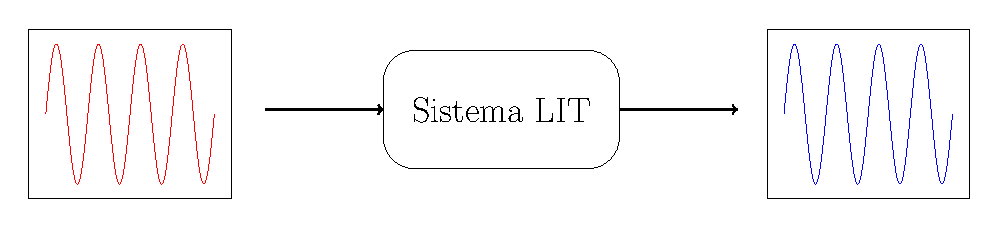
\includegraphics[scale=0.6]{Imagenes/Transformada_Discreta_01.eps}
\end{figure}
\end{frame}
\begin{frame}
\frametitle{Tipos de Transformada}
Series de Fourier.
\\
\bigskip
Señales continuas y periódicas.
\begin{figure}
    \centering
    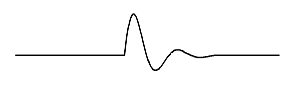
\includegraphics[scale=0.8]{Imagenes/TDF_01.png}
\end{figure}
\end{frame}
\begin{frame}
\frametitle{Tipos de Transformada}
Transformada de Fourier.
\\
\bigskip
Señales continuas y no periódicas.
\begin{figure}
    \centering
    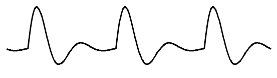
\includegraphics[scale=0.8]{Imagenes/TDF_02.png}
\end{figure}
\end{frame}
\begin{frame}
\frametitle{Tipos de Transformada}
Transformada de Fourier de tiempo discreto.
\\
\bigskip
Señales discretas y no periódicas.
\begin{figure}
    \centering
    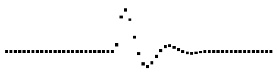
\includegraphics[scale=0.8]{Imagenes/TDF_03.png}
\end{figure}
\end{frame}
\begin{frame}
\frametitle{Tipos de Transformada}
Transformada de Fourier discreta.
\\
\bigskip
Señales discretas y periódicas.
\begin{figure}
    \centering
    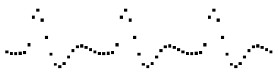
\includegraphics[scale=0.8]{Imagenes/TDF_04.png}
\end{figure}
\end{frame}
\begin{frame}
\frametitle{Primera complicación en el estudio}
Las ondas senoidales (o cosenoidales) están definidas en el intervalo $(-\infty, \infty)$.
\\
\bigskip
\pause
¿Cómo se analiza un conjunto de muestras finito?
\end{frame}
\begin{frame}
\frametitle{La complicación}
No es posible utilizar un conjunto de señales infinitas para analizar una señal de duración finita.
\begin{figure}
    \centering
    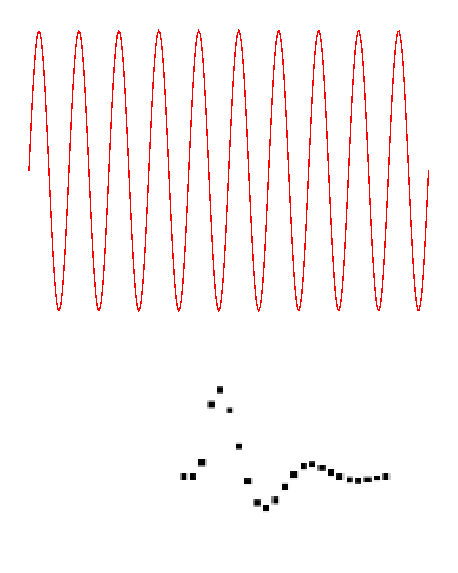
\includegraphics[scale=0.6]{Imagenes/Transformada_Discreta_02.eps}
\end{figure}
\end{frame}
\begin{frame}
\frametitle{¿Cómo se resuelve esta complicación?}
La solución es hacer que la señal \emph{parezca infinita}.
\\
\bigskip
\pause
Veamos dos alternativas para ello.
\end{frame}
\begin{frame}
\frametitle{Primera propuesta: señal discreta y aperiódica}
Se extiende la señal:
\begin{figure}
    \centering
    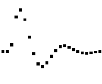
\includegraphics[scale=0.9]{Imagenes/TDF_06.png}
\end{figure}
\pause
Con muestras de valor cero:
\begin{figure}
    \centering
    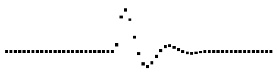
\includegraphics[scale=0.9]{Imagenes/TDF_03.png}
\end{figure}
\end{frame}
\begin{frame}
\frametitle{Segunda propuesta: señal discreta y periódica}
Se extiende la señal:
\begin{figure}
    \centering
    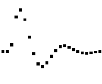
\includegraphics[scale=0.9]{Imagenes/TDF_06.png}
\end{figure}
\pause
repitiendo las muestras reales:
\begin{figure}
    \centering
    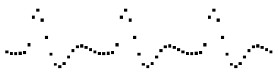
\includegraphics[scale=0.9]{Imagenes/TDF_04.png}
\end{figure}
\end{frame}
\begin{frame}
\frametitle{¿Cómo se calcula la TF computacionalmente?}
Se necesita de infinitas ondas senoidales para analizar una señal no periódica.
\\
\bigskip
\pause
Pero una computadora solo puede trabajar con \emph{señales discretas y finitas}, por lo que la única transformada que se utiliza en el procesamiento y análisis de señales es la Transformada Discreta de Fourier.
\end{frame}

\section{La Transformada Discreta de Fourier}
\frame{\tableofcontents[currentsection, hideothersubsections]}
\subsection{Definición}

\begin{frame}
\frametitle{Expresión de la DFT}
La forma más general de la DFT es:
\begin{align*}
X[k] = \dfrac{1}{N} \nsum_{n=0}^{N-1} x[n] \, \exp(-i \, 2 \, \pi \, k \, n / N)
\end{align*}
\pause
donde:
\setbeamercolor{item projected}{bg=blue!70!black,fg=yellow}
\setbeamertemplate{enumerate items}[circle]
\begin{enumerate}[<+->]
\item $X[k]$ es un número complejo que representa un elemento de la DFT.
\item $x[n]$ es un número complejo que representa un elemento de la señal.
\end{enumerate}
\end{frame}
\begin{frame}
\frametitle{Sobre las operaciones a realizar}
El cálculo de cada punto de la DFT implica $N$ multiplicaciones complejas y $(N {-} 1)$ sumas complejas.
\\
\bigskip
\pause
Por tanto, los $N$ puntos de la DFT pueden obtenerse tras $N^{2}$ multiplicaciones complejas y
$N (N {-} 1)$ sumas complejas.
\end{frame}
\begin{frame}
\frametitle{Modificando la expresión para la DFT}
La expresión para la DFT se puede expresar de la siguiente manera:
\begin{align*}
X[k] = \dfrac{1}{N} \nsum_{n=0}^{N-1} x[n] \, W_{N}^{k \, n}
\end{align*}
donde:
\begin{align*}
W_{N} = \exp(-i \, 2 \, \pi / N)
\end{align*}
\end{frame}
\begin{frame}
\frametitle{Definición de vectores}
Sean los vectores:
\setbeamercolor{item projected}{bg=blue!70!black,fg=yellow}
\setbeamertemplate{enumerate items}[circle]
\begin{enumerate}
\item  $x_{N}$ de $N$ puntos de la secuencia $x[n]$ con $n = 0, 1, \ldots, N-1$
\begin{align*}
x_{n} = \mqty[
x_{0} \\
x_{1} \\
\vdots \\
x_{n-1} \\
]
\end{align*}
\seti
\end{enumerate}
\end{frame}
\begin{frame}
\frametitle{Definición de vectores}
\setbeamercolor{item projected}{bg=blue!70!black,fg=yellow}
\setbeamertemplate{enumerate items}[circle]
\begin{enumerate}[<+->]
\conti    
\item $X_{N}$ de $N$ puntos de la muestra en frecuencias $X[N]$.
\begin{align*}
X_{n} = \mqty[
X_{0} \\
X_{1} \\
\vdots \\
X_{n-1} \\
]
\end{align*}
\end{enumerate}
\end{frame}
\begin{frame}
\frametitle{Una matriz importante}
Sea la matriz $W_{N}$, una matriz de $N \times N$:
\begin{align*}
W_{N} =
\mqty[
1 & 1 & 1 & \ldots & 1 \\
1 & W_{N} & W_{N}^{2} & \ldots & W_{N}^{N-1} \\
1 & W_{N}^{2} & W_{N}^{4} & \ldots & W_{N}^{2(N-1)} \\
\vdots & \vdots & \vdots & \vdots & \vdots \\
1 & W_{N}^{N-1} & W_{N}^{2(N-1)} & \ldots & W_{N}^{(N-1)(N-1)} \\
]
\end{align*}
\end{frame}
\begin{frame}
\frametitle{Nueva expresión para la DFT}
Con los vectores y matriz definidos, la DFT de $N$ puntos se puede expresar en forma matricial como:
\begin{align*}
X_{N} = W_{N} \, x_{N}
\end{align*}
donde $W_{N}$ es la matriz de la transformación lineal. Nótese que $W_{N}$ es una matriz simétrica.
\end{frame}
\begin{frame}
\frametitle{Primer ejemplo}
Calcular la DFT de la secuencia de $4$ puntos:
\begin{align*}
x_{n} = (0, 1, 2, 3)
\end{align*}
\pause
Por lo que habrá que determinar la matriz $W_{4}$, podemos ocupar la propiedad de simetría:
\pause
\begin{align*}
W_{N}^{k + N / 2} = - W_{N}^{k}
\end{align*}
\end{frame}
\begin{frame}
\frametitle{Calculando la matriz}
Entonces la matriz $W_{4}$ es:
\begin{align*}
W_{N} = \mqty[
W_{4}^{0} & W_{4}^{0} & W_{4}^{0} & W_{4}^{0} \\
W_{4}^{0} & W_{4}^{1} & W_{4}^{2} & W_{4}^{3} \\
W_{4}^{0} & W_{4}^{2} & W_{4}^{4} & W_{4}^{6} \\
W_{4}^{0} & W_{4}^{3} & W_{4}^{6} & W_{4}^{9}
 ] {=}
\mqty[
1 & 1 & 1 & 1 \\
1 & W_{4}^{1} & W_{4}^{2} & W_{4}^{3} \\
1 & W_{4}^{2} & W_{4}^{0} & W_{4}^{2} \\
1 & W_{4}^{3} & W_{4}^{2} & W_{4}^{1}
 ] =
\end{align*}
\end{frame}
\begin{frame}
\frametitle{Calculando la matriz}
\begin{align*}
W_{N} = \mqty[
1 & 1 & 1 & 1 \\
1 & -i & -1 & i \\
1 & -1 & 1 & -1 \\
1 & i & -1 & -i
 ]
\end{align*}
\end{frame}
\begin{frame}
\frametitle{El resultado de la DFT}
Entonces se tiene que:
\begin{eqnarray*}
X_{4} = W_{4} \, x_{4} = \pause
\mqty[
1 & 1 & 1 & 1 \\
1 & -i & -1 & i \\
1 & -1 & 1 & -1 \\
1 & i & -1 & -i
 ]
 \cdot [0 \, 1 \, 2 \, 3] = \pause
 \mqty[
6 \\
-2 + 2 \, i \\
-2 \\
-2 - 2 \, j
 ]
\end{eqnarray*}
\end{frame}
\begin{frame}
\frametitle{Algoritmo para un $N$ grande}
Si queremos calcular la DFT de un conjunto discreto de puntos, pero el valor de $N$ es grande, se debe de contar con un algoritmo computacional que optimize el cálculo por el número de operaciones involucradas.
\\
\bigskip
\pause
En lenguajes como \texttt{python}, se incluyen librerías científicas para el cálculo de la DFT.
\end{frame}
\begin{frame}
\frametitle{Librerías científicas}
Las librerías \texttt{numpy} y \texttt{scipy} contienen un conjunto de módulos con funciones matemáticas de alto nivel.
\\
\bigskip
\pause
En particular el módulo \texttt{scipy.fftpack} contiene la función que calcula la transformada rápida de Fourier, que es la que ocuparemos en los siguientes ejemplos.
\end{frame}

\section{Ejercicios computacionales}
\frame{\tableofcontents[currentsection, hideothersubsections]}
\subsection{Ejemplo 1 - Puntos discretos}

\begin{frame}
\frametitle{Cálculo de la DFT}
Calcular la DFT para el siguiente conjunto de puntos:
\begin{align*}
x_{n} = [0, \, 1, \, 2, \, 3, \, 4] 
\end{align*}
En comparación del ejemplo \enquote{a mano}, se tiene un punto más en la secuencia, pero el tamaño de la matriz $W_{N}$ aumenta.
\end{frame}
\begin{frame}[fragile, allowframebreaks]
\frametitle{Código en \texttt{python}}
En \texttt{python ocupamos el siguiente código}:
\begin{lstlisting}
import numpy as np
import scipy.fftpack as fourier

xn = [0, 1, 2, 3, 4] 
Xk = fourier.fft(xn) 

print('DFT: ', Xk)

# Calculamos la Magnitud de la FFT
M_Xk = abs(Xk)   

# Calculamos la Fase de la FFT
Ph_Xk = np.angle(Xk)

print('Magnitud: ', M_Xk)
print('Angulo: ', Ph_Xk*180/np.pi)
\end{lstlisting}
\end{frame}
\begin{frame}[fragile]
\frametitle{Al ejecutar el código se obtiene}
\pause
\begin{verbatim}
DFT: [10. -0.j  -2.5+3.4409548j  
-2.5+0.81229924j -2.5  -0.81229924j
-2.5-3.4409548j]

Magnitud: [10.  4.25325404  2.62865556
  2.62865556  4.25325404]

Angulo: [  -0. 126. 162. -162. -126.]
\end{verbatim}
\end{frame}

\subsection{Ejemplo 2 - Una señal compuesta}
\begin{frame}
\frametitle{Una señal compuesta con más datos}
Vamos a generar una una señal compuesta por dos ondas sinusoidales de $\SI{60}{\hertz}$ y de $\SI{223}{\hertz}$, con $1000$ puntos.
\\
\bigskip
\pause
Le vamos a incorporar \enquote{ruido} a la señal compuesta y luego mediante la FFT se identificarán las frecuencias predominantes de la señal.
\end{frame}
\begin{frame}
\frametitle{Primera señal $w_{1}$}
\begin{figure}
    \centering
    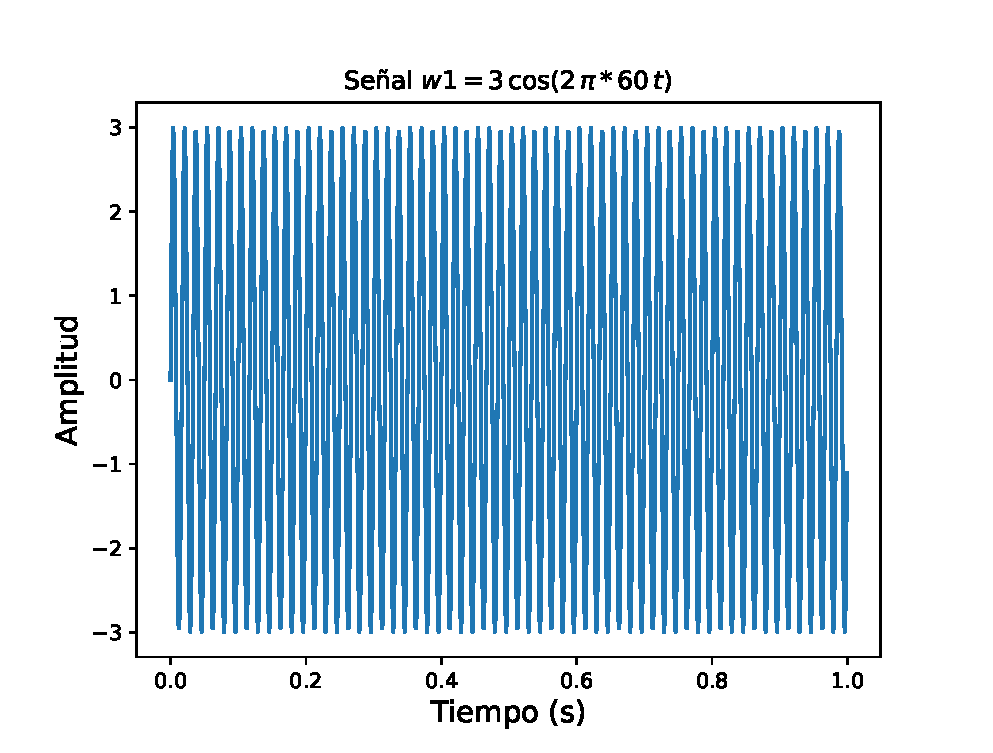
\includegraphics[scale=0.65]{Imagenes/DFT_Analisis_Senal_01.eps}
\end{figure}
\end{frame}
\begin{frame}
\frametitle{Segunda señal $w_{2}$}
\begin{figure}
    \centering
    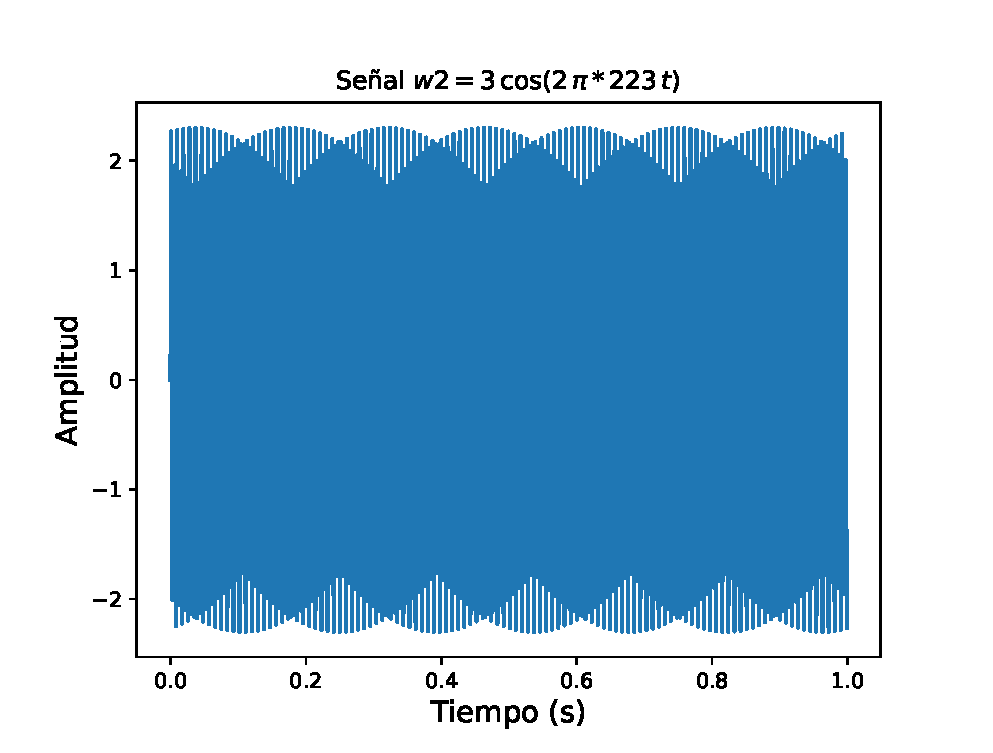
\includegraphics[scale=0.65 ]{Imagenes/DFT_Analisis_Senal_02.eps}
\end{figure}
\end{frame}
\begin{frame}[fragile]
\frametitle{Obteniendo la señal compuesta}
Para generar la señal compuesta, hacemos que:
\begin{lstlisting}
Ts = 0.001
Fs = 1/Ts
n = Ts*np.arange(0, 1000)

w1 = 3*np.sin(2*np.pi*60*n)
w2 = 2.3*np.sin(2*np.pi*223*n)

ruido = np.random.random(len(n))
xn = w1 + w2 + ruido 
\end{lstlisting}
\end{frame}
\begin{frame}
\frametitle{Señal compuesta: $w_{1} + w_{2} +$ ruido}
\begin{figure}
    \centering
    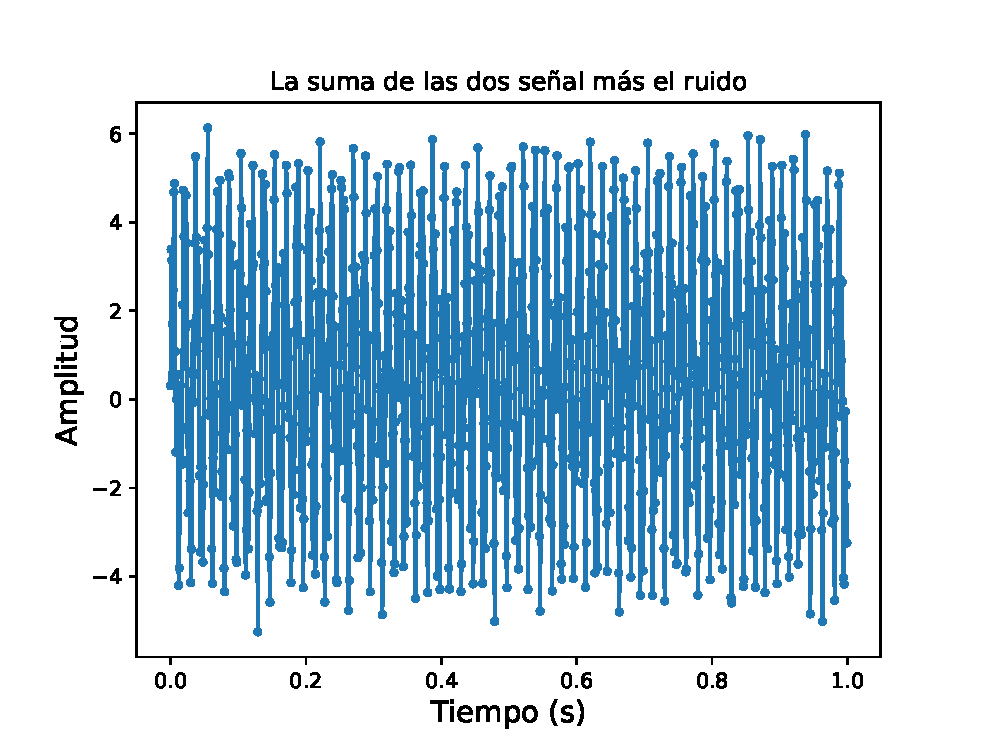
\includegraphics[scale=0.6]{Imagenes/DFT_Analisis_Senal_03.eps}
\end{figure}
\end{frame}
\begin{frame}[fragile]
\frametitle{Obtenemos el espectro de frecuencias}
\begin{lstlisting}
Xk = fourier.fft(xn)
M_Xk = abs(Xk)

F = Fs*np.arange(0, len(xn))/len(xn)
\end{lstlisting}
Incorporamos una rutina de graficación:
\end{frame}
\begin{frame}
\frametitle{Espectro de frecuencias con la DFT}
\begin{figure}
    \centering
    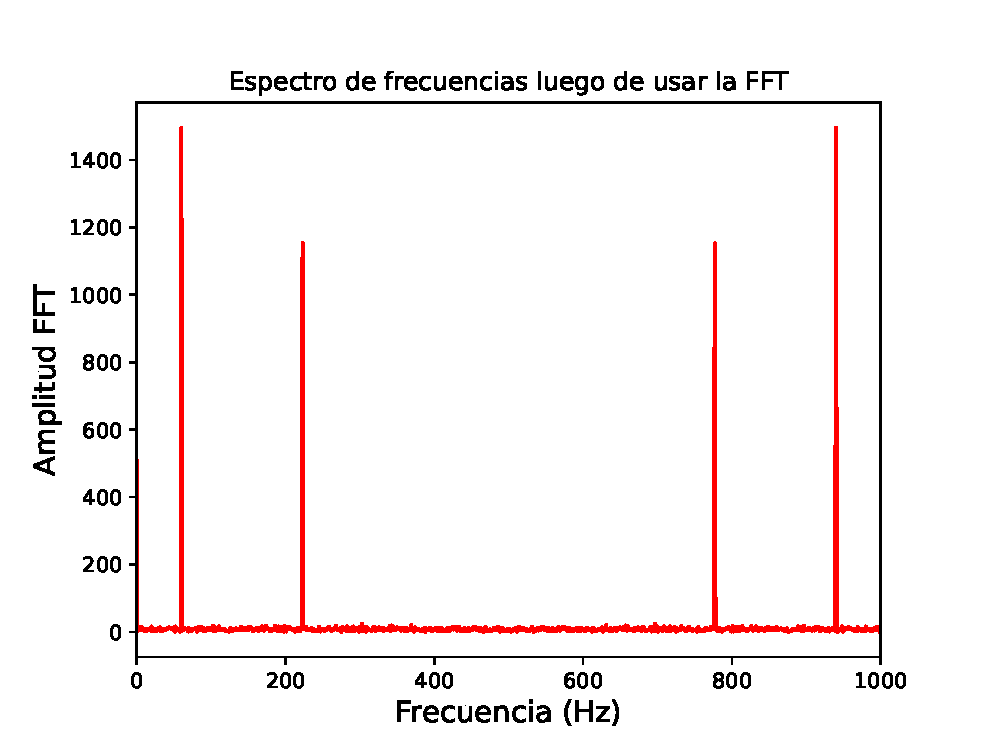
\includegraphics[scale=0.6]{Imagenes/DFT_Analisis_Senal_04.eps}
\end{figure}
\end{frame}
\begin{frame}
\frametitle{Resultados}
\setbeamercolor{item projected}{bg=blue!70!black,fg=yellow}
\setbeamertemplate{enumerate items}[circle]
\begin{enumerate}[<+->]
\item La gráfica es simétrica, por lo que podemos ocupar la parte izquierda de la misma.
\item Las frecuencias dominantes en la señal son: $\SI{60}{\hertz}$ y $\SI{223}{\hertz}$
\item Estos resultados ya los conocíamos de antemano, por la definición de las señales primarias $w_{1}$ y $w_{2}$.
\end{enumerate}
\end{frame}

\subsection{Ejemplo 3 - Una nota musical}

\begin{frame}
\frametitle{Ejemplo 3: Variante en la señal de entrada}
El ejemplo que veremos considera una señal de audio, obtenida al \enquote{pisar} la cuerda en una guitarra clásica para recuperar la nota \emph{Sol}.
\\
\bigskip
\pause
En \texttt{python} existen librerías para el análisis de señales en distintos formatos, en este caso, con un archivo \texttt{*.wav}.
\end{frame}
\begin{frame}[fragile]
\frametitle{La señal de entrada}
Al ocupar las librerías:
\begin{verbatim}
import scipy.io.wavfile as waves
import winsound
\end{verbatim}
Toma en cuenta que la librería \texttt{winsound} funciona bien en entornos \emph{Windows}.
\end{frame}
\begin{frame}
\frametitle{El archivo con la nota musical}
Debido a un conflicto con el formato del archivo, ya que Beamer reproduce archivos mp3, y el de la nota musical está en formato wav, te pedimos descargues el archivo y lo dejes en la misma carpeta donde tengas este documento pdf.
\\
\bigskip
La idea es que escuches la nota y asocies los resultados encontrados.
\end{frame}
% \begin{frame}
% \frametitle{Enlace al archivo de audio}

% \sound{Hola Audio}{Audios/rec_SOL.wav}

% \end{frame}
\begin{frame}
\frametitle{La nota en la guitarra}
Al recuperar los valores de la señal de audio, graficamos los mismos para visualizar la nota \emph{Sol}, como se presenta en la siguiente diapositiva:
\end{frame}
\begin{frame}
\frametitle{Gráfica de la nota musical}
\begin{figure}
    \centering
    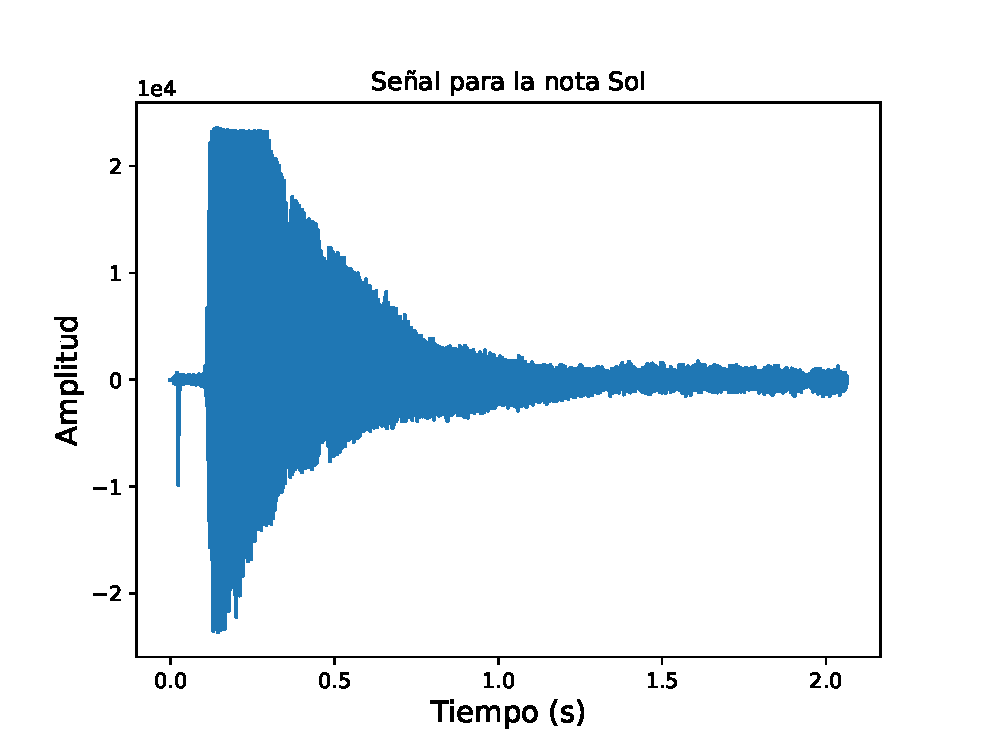
\includegraphics[scale=0.6]{Imagenes/DFT_Analisis_Senal_Audio_01.eps}
\end{figure}
\end{frame}
\begin{frame}
\frametitle{Análisis de la señal}
Una vez recuperados los puntos de la señal:
\setbeamercolor{item projected}{bg=blue!70!black,fg=yellow}
\setbeamertemplate{enumerate items}[circle]
\begin{enumerate}[<+->]
\item A partir de la longitud de la señal: $91008$ puntos, se define un vector de tiempo de la misma longitud.
\item Se calcula la DFT.
\item Se obtiene la magnitud de la DFT.
\item Configuramos el entorno gráfico para una mejor visualización.
\item Con el algoritmo se determina la magnitud máxima de la frecuencia.
\end{enumerate}
\end{frame}
\begin{frame}
\frametitle{Gráfica del espectro de frecuencias}
\begin{figure}
    \centering
    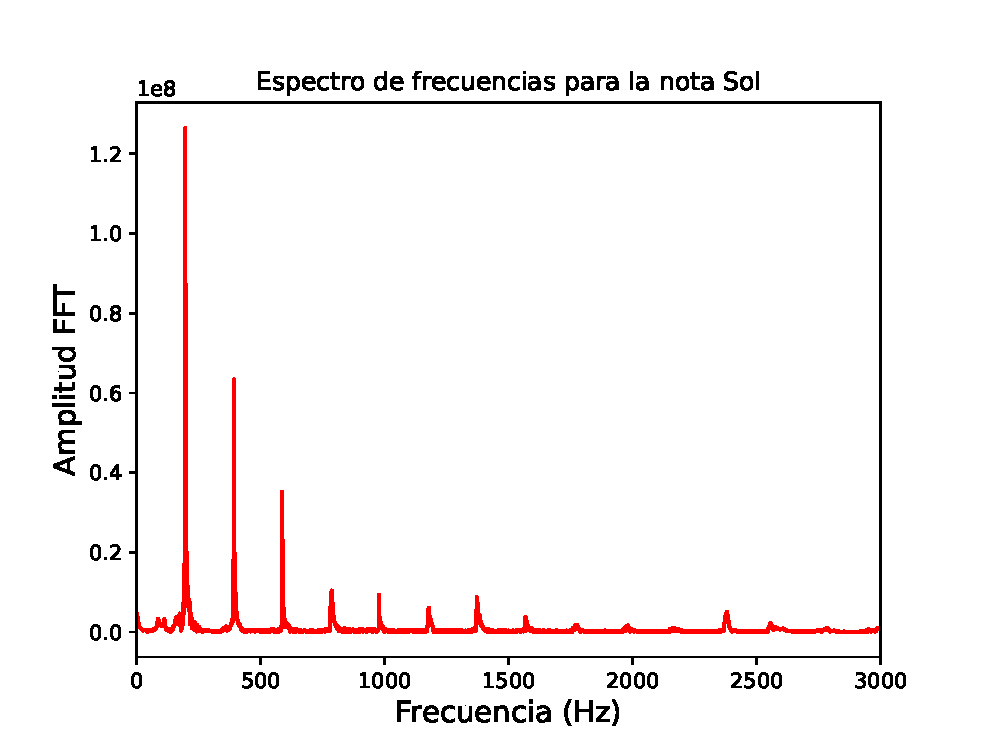
\includegraphics[scale=0.6]{Imagenes/DFT_Analisis_Senal_Audio_02.eps}
\end{figure}
\end{frame}
\begin{frame}
\frametitle{Resultados del análisis}
\setbeamercolor{item projected}{bg=blue!70!black,fg=yellow}
\setbeamertemplate{enumerate items}[circle]
\begin{enumerate}[<+->]
\item La frecuencia dominante de la nota \emph{Sol} es: $\SI{195.767}{\hertz}$.
\item De la gráfica del espectro de frecuencias se identifican los armónicos de la señal.
\end{enumerate}
\end{frame}

\subsection{Ejemplo 4 - Análisis en tiempo real}

\begin{frame}
\frametitle{Análisis espectral}
Haremos ahora el análisis espectral en tiempo real usando como entrada un micrófono (HyperX SoloCast).
\\
\bigskip
\pause
En este formato de videoconferencia se complica el registro de la señal, por lo que se grabó en tiempo real cada muestra y los resultados del análisis del cálculo de la DFT se muestran al mismo tiempo.
\end{frame}
\begin{frame}
\frametitle{Ajustes en \texttt{python}}
Se ocuparán otras librerías y se ajustará el entorno gráfico en \texttt{python} para mostrar en una misma ventana, dos subgráficas:
\setbeamercolor{item projected}{bg=blue!70!black,fg=yellow}
\setbeamertemplate{enumerate items}[circle]
\begin{enumerate}[<+->]
\item En la parte superior la señal de entrada tomada del micrófono (puerto USB)
\item En la parte inferior, el espectro de frecuencias en tiempo real.
\end{enumerate}
\end{frame}
\begin{frame}
\frametitle{Aclaraciones importantes}
Con el micrófono externo se graba la señal directamente, pero también hay ruido ambiental, por lo se notará de repente, cambios en la señal de entrada.
\\
\bigskip
\pause
Por la grabación se presenta un \emph{lag}, esperamos que no sea tan grande para perder el seguimiento en las señales.
\end{frame}
% \begin{frame}[fragile]
% \frametitle{Muestras de señales}
% \setbeamercolor{item projected}{bg=blue!70!black,fg=yellow}
% \setbeamertemplate{enumerate items}[circle]
% \begin{enumerate}[<+->]
% \item Se hace una lectura en voz alta de un párrafo.
% \item Canción del grupo U2.
% \item Canción del grupo VCMG.
% \item Canción del grupo Maximum The Hormone.
% \item Señales con generador de audio.
% \end{enumerate}
% \end{frame}
\begin{frame}
\frametitle{Indicaciones}
El archivo \emph{*.wav} y los archivos \emph{*.mp4} deben de estar en la misma carpeta donde se encuentra el pdf, ya que el documento los buscará ahí.
\\
\bigskip
\pause
Dependiendo del sistema operativo que estés utilizando, se seleccionará el programa por defecto para reproducir el audio.
\end{frame}
\begin{frame}
\frametitle{Indicaciones}
Haz click sobre la imagen \emph{MP4}, y se abrirá de manera independiente el reproductor de audio, en caso de que no se inicie la reproducción, basta con que presiones el botón \emph{play} del reproductor.
\\
\bigskip
\pause
Una vez que la reproducción se haya completado, cierra el reproductor de audio y continua con la presentación en pdf.
\end{frame}
\begin{frame}
\frametitle{Lectura en voz alta de un párrafo}
\begin{figure}
    \centering
    \movie[externalviewer]{

\includegraphics[scale=0.25]{Imagenes/logo_mp4.png}}{Audios/2021_Asesorias_27_DFT_Ejercicios_Audio_01_Lectura.mp4}
\end{figure}
\end{frame}
\begin{frame}
\frametitle{Sobre la lectura en voz alta}
El espectro de frecuencias muestra cambios no tan amplios tanto en la amplitud de la señal como de la frecuencia.
\\
\bigskip
\pause
Se sabe que la frecuencia de la voz de una mujer es diferente a la frecuencia de la voz de un hombre. ¿Qué tanta diferencia en promedio puede haber?
\end{frame}
\begin{frame}
\frametitle{Fragmento canción U2}
\begin{figure}
    \centering
    \movie[externalviewer]{
    
\includegraphics[scale=0.25]{Imagenes/logo_mp4.png}}{Audios/2021_Asesorias_27_DFT_Ejercicios_Audio_02_U2.mp4}
\end{figure}
\end{frame}
\begin{frame}
\frametitle{Sobre el espectro de frecuencias}
El fragmento de la canción consta de tres partes:
\setbeamercolor{item projected}{bg=blue!70!black,fg=yellow}
\setbeamertemplate{enumerate items}[circle]
\begin{enumerate}[<+->]
\item Una entrada tipo de sintonización de estación de radio.
\item Un fragmento de opertura con música de cámara.
\item El comienzo de la canción rock.
\end{enumerate}
\end{frame}
\begin{frame}
\frametitle{Sobre el espectro de frecuencias}
El espectro de frecuencias muestra un comportamiento muy específico en cada parte del fragmento de la canción de U2, en particular, el fragmento de opertura con música de cámara, revela un espectro muy definido donde la señal de entrada consta de bastantes instrumentos musicales de manera simultánea.
\end{frame}
\begin{frame}
\frametitle{Fragmento canción VCMG}
\begin{figure}
    \centering
    \movie[externalviewer]{

\includegraphics[scale=0.25]{Imagenes/logo_mp4.png}}{Audios/2021_Asesorias_27_DFT_Ejercicios_Audio_03_VCMG.mp4}
\end{figure}
\end{frame}
\begin{frame}
\frametitle{Sobre el espectro obtenido}
La canción pertenece al género de música electrónica, cada parte de la misma se construye con sintetizadores, moduladores, software especializado, etc.
\\
\bigskip
\pause
El espectro de la señal de entrada muestra un paquete típico de información compactada, es decir, a diferencia de la señal de voz, de la sintonización de radio y la canción de rock, hay una estructura más definida en la señal.
\end{frame}
\begin{frame}
\frametitle{Fragmento canción Maximum The Hormone}
\begin{figure}
    \centering
    \movie[externalviewer]{

\includegraphics[scale=0.25]{Imagenes/logo_mp4.png}}{Audios/2021_Asesorias_27_DFT_Ejercicios_Audio_04_Maximum.mp4}
\end{figure}
\end{frame}
\begin{frame}
\frametitle{Sobre el espectro de frecuencias}
El fragmento de la canción de género heavy metal, muestra una señal de entrada saturada de sonidos de guitarras eléctricas, batería, bajo y la voz del cantante.
\\
\bigskip
\pause
Cada canción en general se somete a trabajo de edición para agregar efectos o incorporar otros sonidos para hacerlas más atractivas, pero el espectro de frecuencias muestra nuevamente una combinación de las frecuencias dominantes.
\end{frame}
\begin{frame}
\frametitle{Generador de señales}
\begin{figure}
    \centering
    \movie[externalviewer]{

\includegraphics[scale=0.25]{Imagenes/logo_mp4.png}}{Audios/2021_Asesorias_27_DFT_Ejercicios_Audio_05_Generador.mp4}
\end{figure}
\end{frame}
\begin{frame}
\frametitle{Sobre el espectro en el generador}
Se utilizó una señal senoidal que cambia su frecuencia de $\SI{500}{\hertz}$ a $\SI{3}{\kilo\hertz}$, se nota en el espectro de frecuencias que la frecuencia dominante se desplaza precisamente entre estos valores.
\\
\bigskip
\pause
En la última parte se deja una frecuencia fija, por lo que ya no hay desplazamiento en el espectro.
\end{frame}
\begin{frame}
\frametitle{Conclusión}
Los ejemplos presentados a pesar de ser sencillos en la preparación y codificación con \texttt{python}, muestran el potencial estudio de señales de audio mediante la DFT.
\\
\bigskip
\pause
En cada área específica de la física, será posible analizar señales de audio, imágenes, señales fisiológicas, etc. mediante las herramientas matemáticas que se han desarrollado en el semestre.
\end{frame}
\end{document}